\documentclass{article}


\usepackage{standalone}
\usepackage{pgf}
\usepackage{pgfkeys}
\usepackage{gnuplottex}
\usepackage{amssymb}
\usepackage{graphicx}
\usepackage{amsmath}
\usepackage{algorithm}
\usepackage{algorithmicx}
\usepackage{algpseudocode}
\usepackage{pgfplots}
\usepackage{epstopdf}  
\usepackage[utf8]{inputenc}
\usepackage[T1]{fontenc}
\usepackage{graphicx}
\usepackage{amsmath}
\usepackage{makecell}
\usepackage{amssymb}
\usepackage{multicol}
\usepackage{natbib}
\usepackage{hyperref}
\usepackage{booktabs} % For professional quality tables
\usepackage{array}    % For better column alignment
\usepackage{tikz}
\usepackage{pgfkeys}
\usepackage[a4paper, margin=2cm]{geometry}
\usepackage{pgfplots}
\usepackage{epstopdf}  
\usepackage{graphicx}
\usepackage{float}
\usepackage{tikz}
\usepackage{pgf}
\usepackage{pgfkeys}
\usepackage{gnuplottex}
\usepackage{amsmath}

% Sets
\newcommand{\SetWorkOrder}[1]{W(\VarMetaTime#1)}
\newcommand{\ElementWorkOrder}{w}
\newcommand{\SetPeriod}{P(\VarMetaTime)}
\newcommand{\ElementPeriod}{p}

\newcommand{\SetResource}{R(\VarMetaTime)}
\newcommand{\ElementResource}{r}
\newcommand{\SetOperation}[2]{O_{#1}(\VarMetaTime, #2)}
\newcommand{\ElementOperation}{o}

\newcommand{\SetDays}[1]{D_{#1}(\VarMetaTime)}
\newcommand{\ElementDays}{d}
\newcommand{\SetActivity}[2]{A_{#2}(\VarMetaTime, #1)}
\newcommand{\ElementActivity}{a}

\newcommand{\SetWorkSegment}{K(\VarSupervisorAssignment{}{})}
\newcommand{\ElementWorkSegment}{k}
\newcommand{\SetTimeInstance}{I(\VarMetaTime)}
\newcommand{\ElementTimeInstance}{i}

\newcommand{\SetEvent}{E(\VarMetaTime)}
\newcommand{\ElementEvent}{e}

\newcommand{\SetScheduler}{S}
\newcommand{\ElementScheduler}{s}
\newcommand{\SetSupervisor}{Z}
\newcommand{\ElementSupervisor}{z}

\newcommand{\SetTechnician}{T(\VarMetaTime)}
\newcommand{\ElementTechnician}{t}

% Parameters
\newcommand{\ParStrategicValue}{strategic\_value_{\ElementWorkOrder \ElementPeriod}(\VarMetaTime)}
\newcommand{\ParStrategicPenalty}{strategic\_penalty}
\newcommand{\ParClusteringValue}{clustering\_value_{\ElementWorkOrder1, \ElementWorkOrder2}}
\newcommand{\ParStrategicResource}{resource_{\ElementPeriod\ElementResource}(\VarMetaTime)}

\newcommand{\ParStrategicWorkOrderWeight}{work\_order\_work_{\ElementWorkOrder \ElementResource}}
\newcommand{\ParStrategicInclude}{include(\VarMetaTime)}
\newcommand{\ParStrategicExclude}{exclude(\VarMetaTime)}
\newcommand{\ParTacticalValue}{tactical\_value_{\ElementDays\ElementOperation}(\VarMetaTime)}

\newcommand{\ParTacticalPenalty}{tactical\_penalty}
\newcommand{\ParOperationWork}[1]{work_{#1}(\VarMetaTime)}
\newcommand{\ParTacticalResource}{tactical\_resource_{\ElementDays\ElementResource}(\VarMetaTime)}
\newcommand{\ParStartStart}{start\_start_{\ElementOperation1, \ElementOperation2}}

\newcommand{\ParFinishStart}{finish\_start_{\ElementOperation1, \ElementOperation2}}
\newcommand{\ParEarliestStart}{earliest\_start_{\ElementOperation}(\VarMetaTime)}
\newcommand{\ParLatestFinish}{latest\_finish_{\ElementOperation}(\VarMetaTime)}
\newcommand{\ParNumberOfPeople}{number_{\ElementOperation}(\VarMetaTime)}

\newcommand{\ParOperatingTime}{operating\_time_{\ElementOperation}}
\newcommand{\ParDuration}{duration_{\ElementOperation}(\VarMetaTime)}
\newcommand{\ParSupervisorValue}{supervisor\_value_{\ElementActivity \ElementTechnician}(\VarMetaTime, \VarStartOfSegment{t}{}, \VarFinishOfSegment{t}{})} 
\newcommand{\ParFeasible}{feasible_{at}(\VarIncludeActivity{})}
\newcommand{\ParOperationsForWorkOrder}{work\_order\_to\_operations_{\ElementWorkOrder }}

\newcommand{\ParOperationsInWorkOrder}{operations\_in\_work\_order_{\ElementWorkOrder }}
\newcommand{\ParActivitiesForOperation}{activities\_for\_operation_{\ElementOperation}}
\newcommand{\ParLowerActivityWork}{lower\_activity\_work_{\ElementActivity}(\VarMetaTime)}
\newcommand{\ParActivityWork}[1]{activity\_work_{\ElementActivity}(\VarMetaTime, \VarActivityWork{#1})}

\newcommand{\ParPreparation}{preparation_{\ElementActivity1, \ElementActivity2}}
\newcommand{\ParEvent}{event_{\ElementTimeInstance \ElementEvent}}
\newcommand{\ParEventDuration}{duration_{\ElementTimeInstance \ElementEvent}}
\newcommand{\ParConstraintLimit}{constraint\_limit}

\newcommand{\ParTimeWindowStart}{time\_window\_start_{\ElementActivity}(\VarTacticalWork{}{})}
\newcommand{\ParTimeWindowFinish}{time\_window\_finish_{\ElementActivity}(\VarTacticalWork{}{})}
\newcommand{\ParAvailabilityStart}{availability\_start(\VarMetaTime)}
\newcommand{\ParAvailabilityFinish}{availability\_finish(\VarMetaTime)}

% Variables
\newcommand{\VarStrategicWorkOrderAssignment}[2]{\alpha_{#1#2}(\VarMetaTime)}
\newcommand{\VarStrategicExcess}{\epsilon_{\ElementPeriod\ElementResource}(\VarMetaTime)}
\newcommand{\VarTacticalWork}[2]{\beta_{#1#2}(\VarMetaTime)}
\newcommand{\VarTacticalExcess}{\mu_{\ElementResource \ElementDays}(\VarMetaTime)} 

\newcommand{\VarTacticalWorkBinary}[2]{\sigma_{#1#2}(\VarMetaTime)}
\newcommand{\VarTacticalWorkBinaryConsecutive}{\eta_{\ElementDays\ElementOperation}(\VarMetaTime)}
\newcommand{\VarTacticalOperationDifference}{\Delta_{\ElementOperation}(\VarMetaTime)}
\newcommand{\VarSupervisorAssignment}[2]{\gamma_{#1#2}(\VarMetaTime)}

\newcommand{\VarSupervisorAssignmentWhole}{\phi_{\ElementOperation}(\VarMetaTime)}
\newcommand{\VarActivityWork}[1]{\rho_{#1}(\VarMetaTime)}
\newcommand{\VarProcessingTime}{\delta_{\ElementActivity\ElementWorkSegment}(\VarMetaTime)} 
\newcommand{\VarActiveSegment}[2]{\pi_{#1#2}(\VarMetaTime)}

\newcommand{\VarStartOfSegment}[2]{\lambda_{#1#2}(\VarMetaTime)}
\newcommand{\VarFinishOfSegment}[2]{\Lambda_{#1#2}(\VarMetaTime)}
\newcommand{\VarSegmentInRelation}{\omega_{\ElementActivity\ElementWorkSegment\ElementTimeInstance \ElementEvent}(\VarMetaTime)}
\newcommand{\VarIncludeActivity}[1]{\theta_{#1}(\VarMetaTime)}

% Meta variables
\newcommand{\VarMetaTime}{\tau}


\definecolor{red}{HTML}{8A3F3A}
\definecolor{yellow}{HTML}{E0BB3C}
\definecolor{blue}{HTML}{4569E0}
\definecolor{green}{HTML}{17E561}
\definecolor{other}{HTML}{6A939E}

% DTU Colors
\definecolor{dtu-corporate-red}{HTML}{990000}
\definecolor{dtu-white}{HTML}{ffffff}
\definecolor{dtu-black}{HTML}{000000}
\definecolor{dtu-blue}{HTML}{2F3EEA}
\definecolor{dtu-bright-green}{HTML}{1FD082}
\definecolor{dtu-navy-blue}{HTML}{030F4F}
\definecolor{dtu-yellow}{HTML}{F6D04D}
\definecolor{dtu-orange}{HTML}{FC7634}
\definecolor{dtu-pink}{HTML}{F7BBB1}
\definecolor{dtu-grey}{HTML}{DADADA}
\definecolor{dtu-red}{HTML}{E83F48}
\definecolor{dtu-green}{HTML}{008835}
\definecolor{dtu-purple}{HTML}{79238E}


\begin{document}

\section{Agenda}
\begin{itemize}
	\item Current Situation    (25 min)
    \item Envisioned future    (25 min)
    \item Company Structure    (10 min)
    \item Convincing Total     (25 min)	
    \item IP concerns          (25 min)
    \item Milestones           (15 min)
\end{itemize}

\section{Current Situation}


\begin{itemize}
    \item Manually sending email around
    \item State duplication
    \item SAP is not made for/cannot handle optimization workflows. -> you copy the current SAP state to a file (excel) to continue working from there.
    \item The idea with Ordinator is to be a layer between SAP and the scheduler/supervisor. Ordinator then holds all state which can be manipulated (plannings, optimizations etc.).
\end{itemize}



\begin{figure}[H]
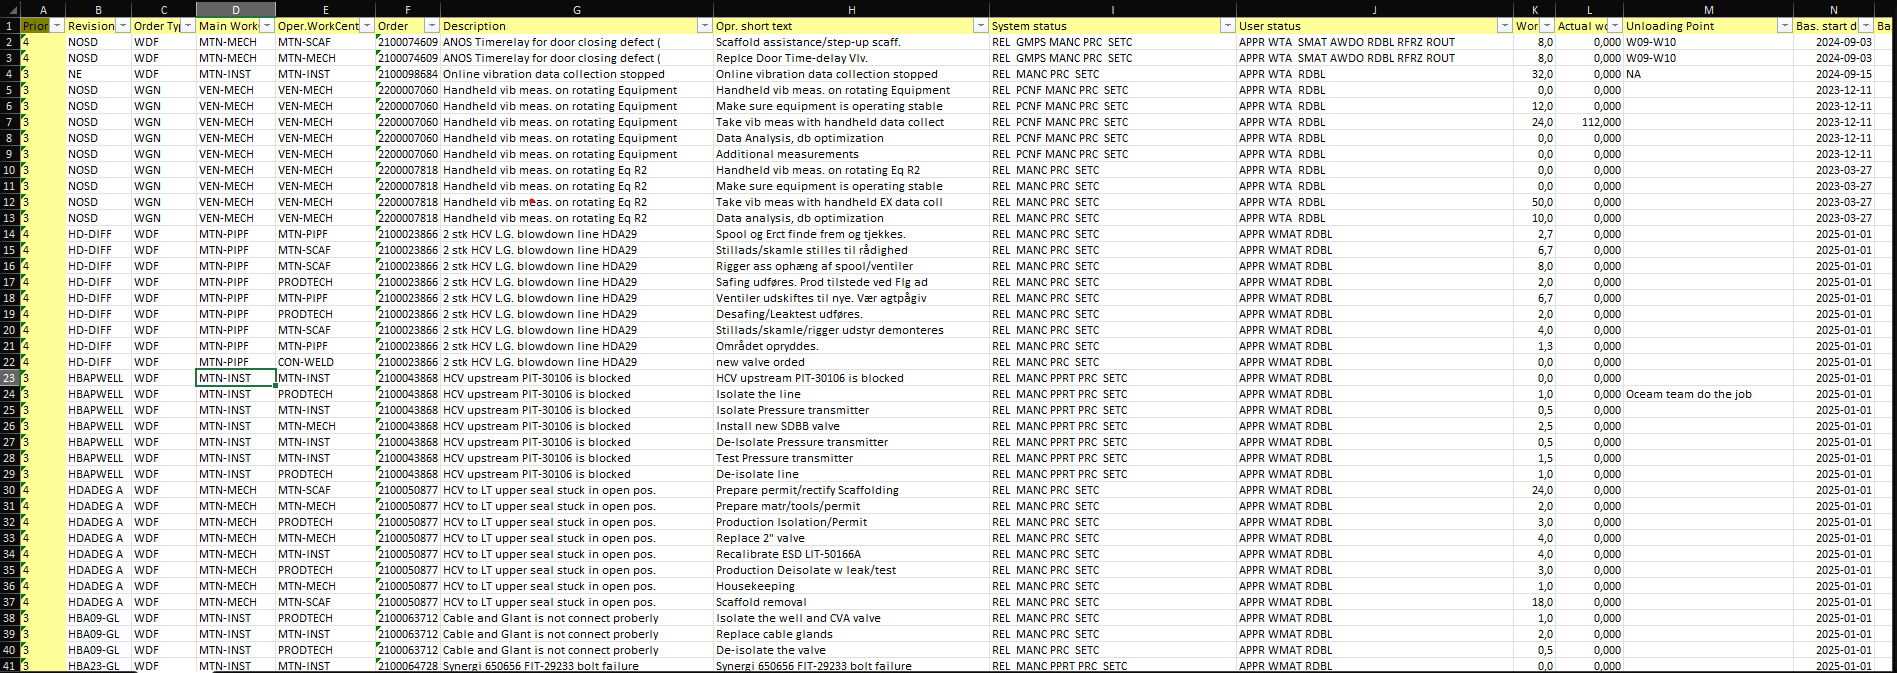
\includegraphics[width=1.0\textwidth]{../../project-plans/scipo-total/figures/schedulers-view-into-the-scheduling-process.png}
\caption{Schedulers view of the scheduling process}
\end{figure}
\begin{figure}[H]
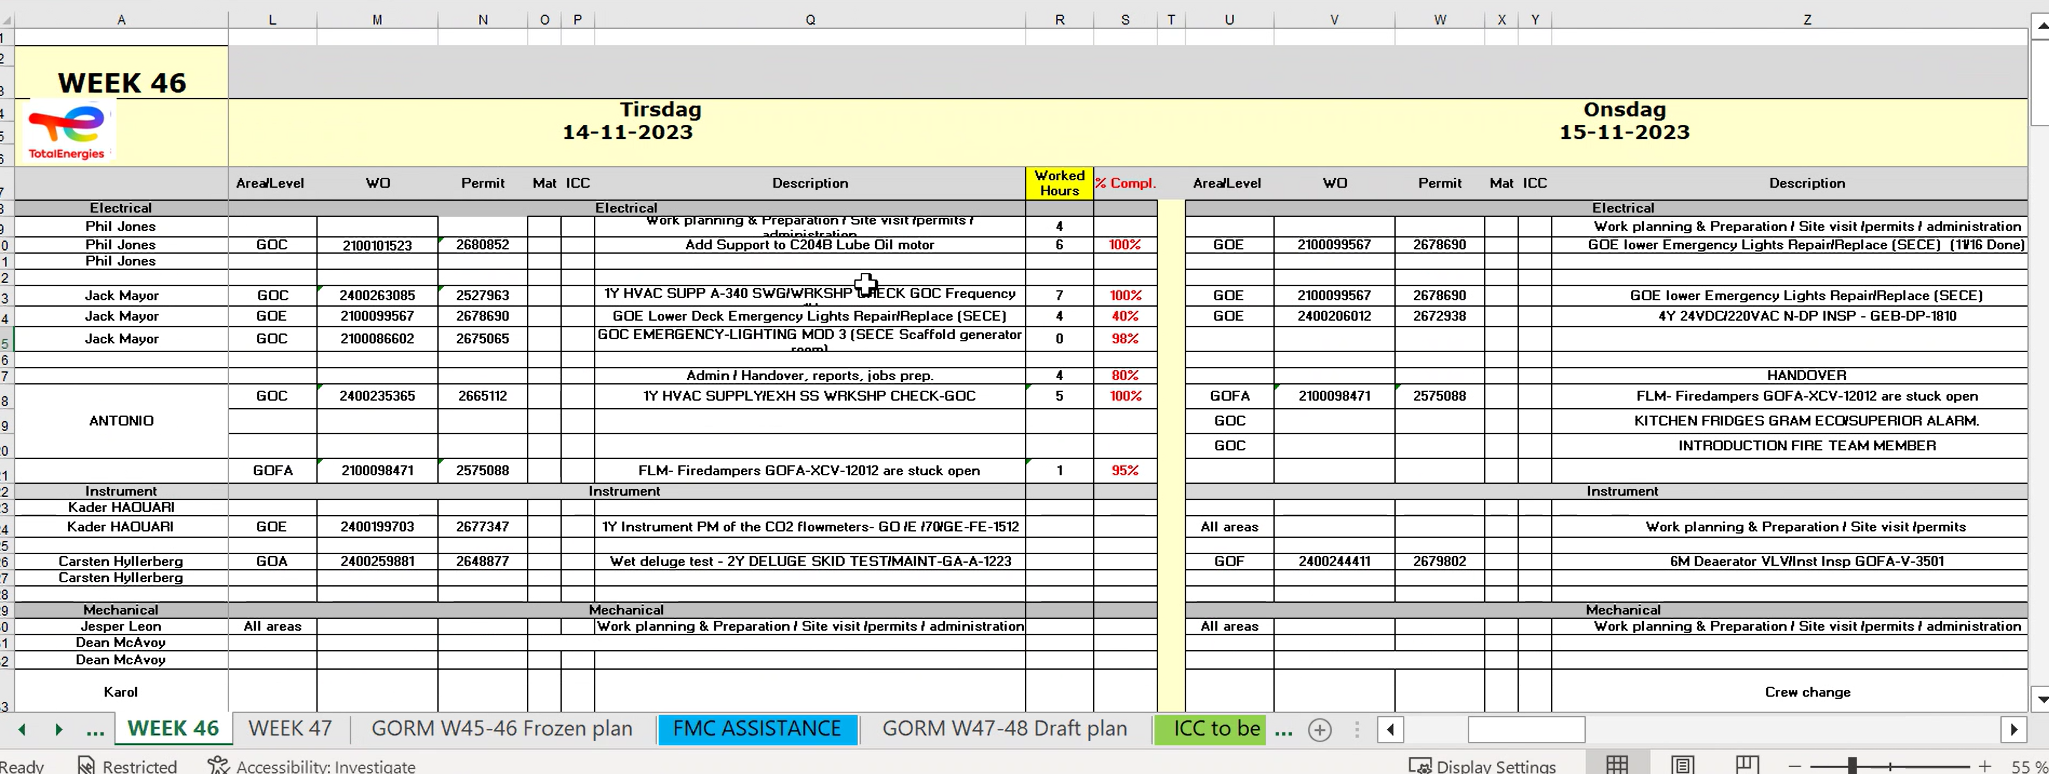
\includegraphics[width=1.0\textwidth]{../../project-plans/scipo-total/figures/technician-excel.png}
\caption{Supervisors and Technicians view of the scheduling process}
\end{figure}
\section{Envisioned Future}

\begin{figure}[H]
    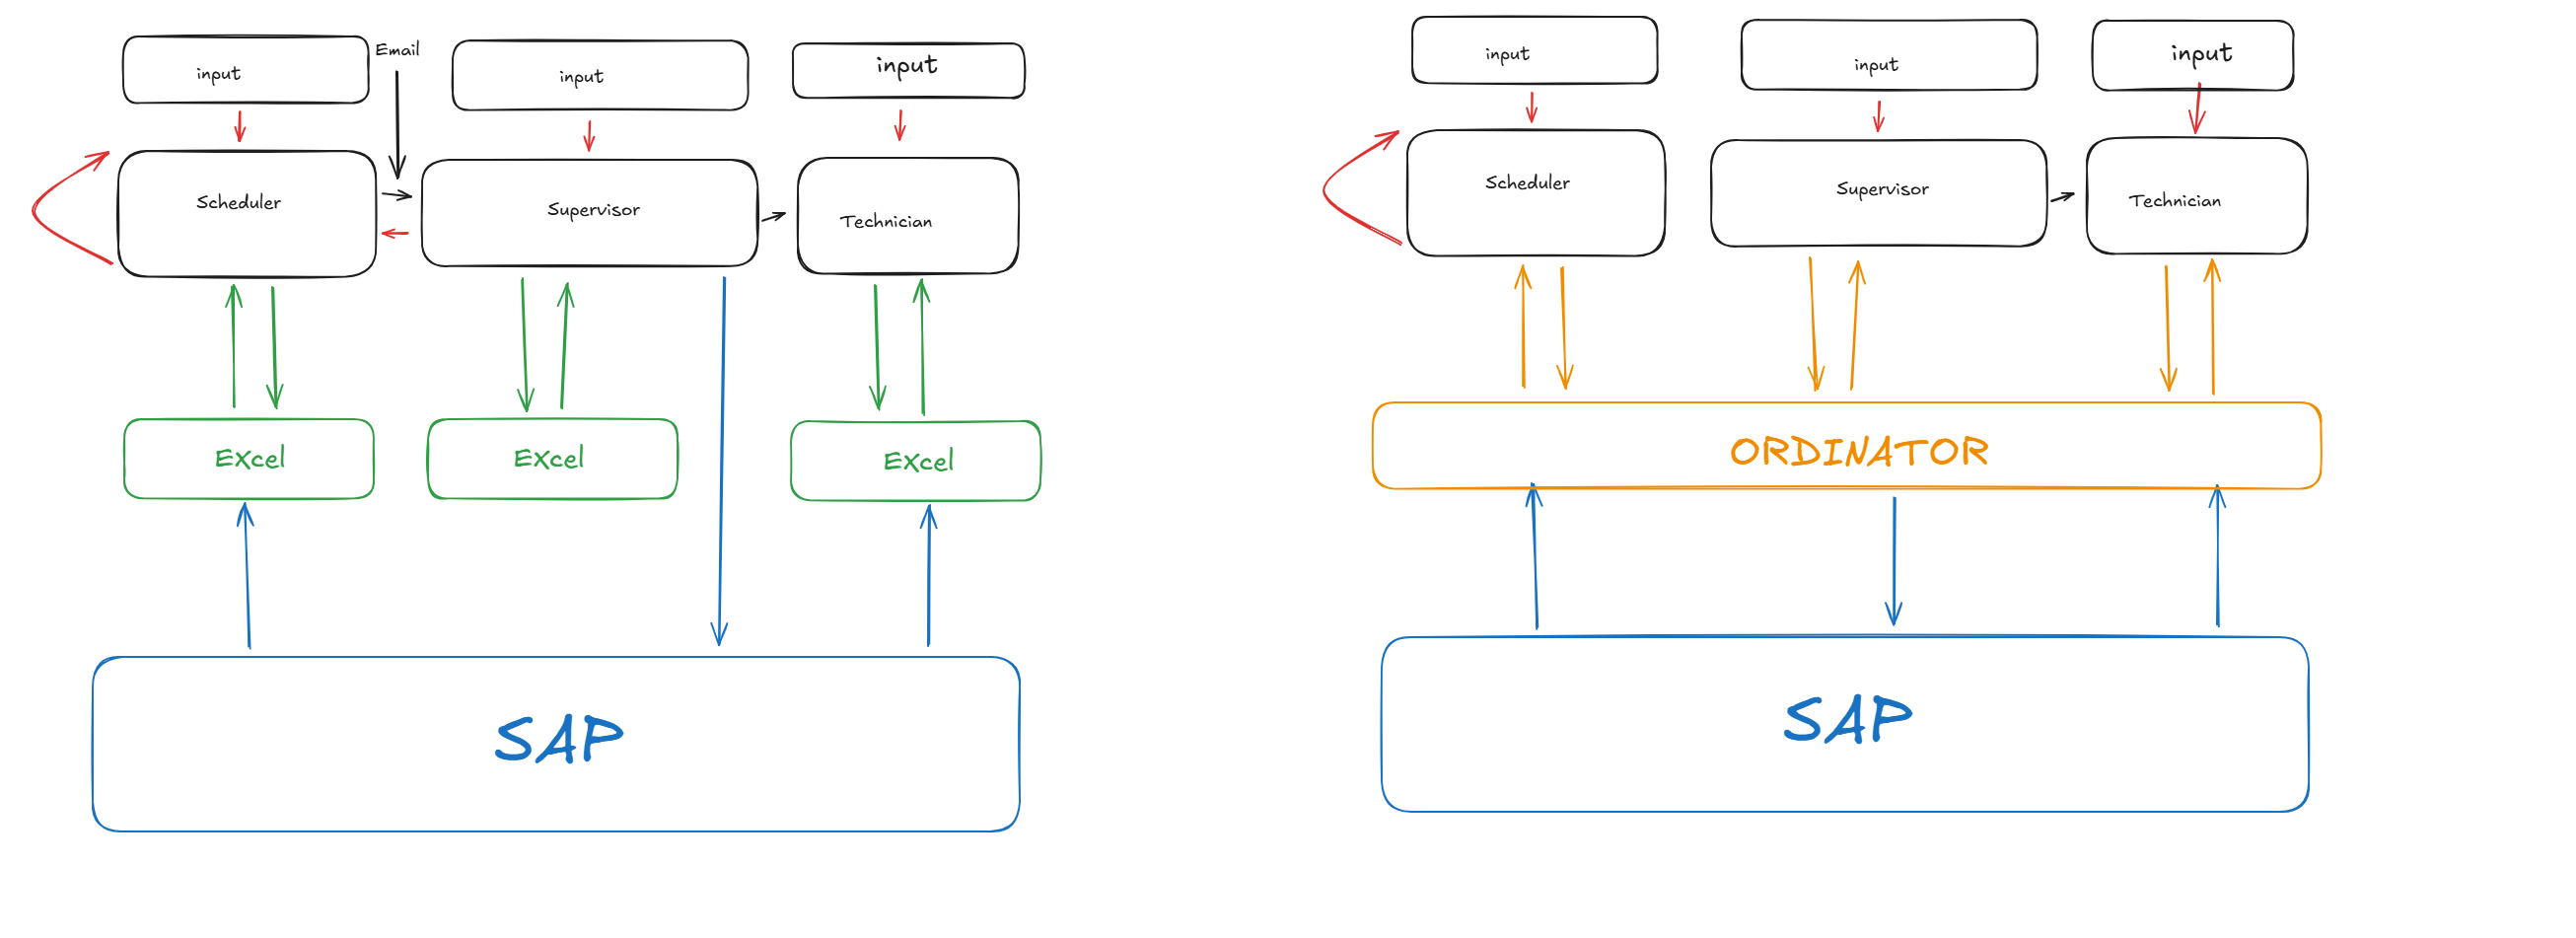
\includegraphics[width=1.0\textwidth]{../../project-plans/scipo-total/figures/scheduling-as-is-to-be.png}
    \caption{Schematic difference between the current way of doing things versus how it could be done in the
    future. Each stakeholder can immediately sees an optimized schedule based on the state in the optimization
    algorithms. This means that the moment that a \textbf{Scheduler}, \textbf{Supervisor}, or \textbf{Technician}
    sees that there is something wrong his part of the schedule it can be handled immediately. After an excel file
    has been sent in the as-is example the remaining stakeholders are working blind}
\end{figure}

\subsection{What do we not know:}
\begin{itemize}
    \item Supervisor is a big unknown. How do they work with the information? Do all supervisors do the same?
    \item Do they know what would be the best for them? DO we?
    \item What should be the main focus to get a minimum viable product?
    \item How mature the "engine" (ordinator) should be before trying to convince TotalEnergies?
\end{itemize}


\section{Possible Company Structure}
Creating a company splitting the shares equally between the founders giving Niels Henrik a 10\% share. 

\subsection{questions}
\begin{itemize}
    \item Should Total own anything?
    \item Does DTU need to own anything?
    % \item Should there be a policy between risk taking and the amount of shares given to a person?
    % \item Where should the company have headquarters?
\end{itemize}

\subsection{IP Concerns}
\begin{itemize}
    \item What rights do DTU have to software?
    \item Do we have a case where DTU are not willing to further this project alone and therefore we can do it ourselves without them?
    \item What does TotalEnergies expect? Do they expect this to be free or are they willing to fund this project even though it would be through a "subcontractor"?
\end{itemize}

\section{Convincing Total}
\begin{itemize}
    \item How to make Total commit themselves to spend hours on the project.
    \begin{itemize}
        \item What does this mean for who owns what?
    \end{itemize}
    \item Booking a meeting with the most relevant stakeholders, and getting a consensus on the project goals.
    \item Drafting a budget, meaning how many hours there is needed to deliver certain milestones.
    \item Working on an hourly basis, delivering weekly or monthly results.
    \item What should the role of Christian's Ph.D. project be until we are ready to create the company?
    \item One route (best-case-scenario): 
    \begin{itemize}
        \item Christian takes leave of PhD in Autumn
        \item Total Energies hopefully is willing to pay for hours in development
        \item Christian and Sebastian works full time on paid project to develop
        \item Christian returns to finish PhD or project is so mature we cannot stop now.
    \end{itemize}
\end{itemize}

\subsection{Budget}


\begin{table}[H]

\centering
\begin{tabular}{lllllll}
    \toprule
    \textbf{Scipo}                                                          & Role                            & \makecell[lt]{Total\\Hours} & \makecell[lt]{Cost per\\Hour}        & Skills                                                                  & Period                             &  \\
    \midrule
    Christian Jespersen                                                     & \makecell[lt]{Core\\Developer}  & 320                         & 250 DKK                              & \makecell[lt]{Optimization\\Algorithms}                                 & \makecell[lt]{2025-09 to\\2025-12} &  \\
    Sebastian Dall                                                          & \makecell[lt]{Core\\Developer}  & 320                         & 250 DKK                              & \makecell[lt]{API,\\Frontend,\\Project}                                 & \makecell[lt]{2025-09 to\\2025-12} &  \\
    \toprule
    \textbf{Total}                                                          & Role                            & \makecell[lt]{Total\\Hours} & \makecell[lt]{Cost per\\Hour}        & Skills                                                                  & Period                             &  \\
    \midrule
    \makecell[tl]{TOTAL\_DEVELOPER\\Baptiste Dubillaud}                     & Integration                     & 50-70                       & 500 DKK                              & \makecell[lt]{Azure,\\IT infrastructure}                                & \makecell[lt]{2025-09 to\\2025-12} &  \\
    \makecell[tl]{TOTAL\_MAINTENANCE\_METHOD\\Brian Friis Niels}            & Domain Expert                   & 40                          & 500 DKK                              & \makecell[lt]{Understanding of\\Business Flows}                            & \makecell[lt]{2025-09 to\\2025-12} &  \\
    \makecell[tl]{GMC\_SCHEDULER\\Valentin Ispas}                           & Domain Expert                   & 30                          & 500 DKK                              & \makecell[lt]{Key Stakeholder}                                          & \makecell[lt]{2025-09 to\\2025-12} &  \\
    \makecell[tl]{GMC\_SUPERVISOR\\<UNKNOWN>}                               & Domain Expert                   & 20                          & 500 DKK                              & \makecell[lt]{Key Stakeholder}                                          & \makecell[lt]{2025-09 to\\2025-12} &  \\
    \makecell[tl]{GMC\_TECHNICIAN\\<UNKNOWN>}                               & Domain Expert                   & 20                          & 500 DKK                              & \makecell[lt]{Key Stakeholder}                                          & \makecell[lt]{2025-09 to\\2025-12} &  \\
    \toprule
    \textbf{Material}                                                       & Role                            & \makecell[lt]{Total\\Hours} & \makecell[lt]{Cost per\\Hour}        & Skills                                                                  & Period                             &  \\
    \midrule
    Server                                                                  & -                               & ~2000                       & ~1-5 DKK                             & -                                                                       & \makecell[lt]{2025-09 to\\2025-12} &  \\
    \bottomrule
\end{tabular}

\end{table}

\[
\begin{aligned}
    \text{Total Cost} &= (320 \times 250) + (320 \times 250) \\
    &\quad + (70 \times 500) + (40 \times 500) + (30 \times 500) \\
    &\quad + (20 \times 500) + (20 \times 500) + (2,000 \times 5) \\
    &= 80,000 + 80,000 + 35,000 + 20,000 + 15,000 + 10,000 + 10,000 + 10,000  \\
    &= 160,000 \quad (\text {Direct cost for Scipo}) \\
    &\quad + 100,000 \quad (\text {Indirect cost for Total}) \\
    &= 260,000 \quad \text{Total cost DKK}
\end{aligned}
\]

Total cost per 2 month period \textbf{260,000 DKK}

\section{Appendix}

\usetikzlibrary {positioning}
\newcommand{\drawHexagon}[6][draw=black]{
	\draw[#1, fill=#4] (#2,#3) ++(30:#6) -- ++(90:#6) -- ++(150:#6) -- ++(210:#6) -- ++(270:#6) -- ++(330:#6) -- cycle;
	\node[align=center] at (#2,#3+2) {#5};
}

\newif\ifpersistencelayer
\newif\ifatomicpointerswaplayer
\newif\ifmetaheuristicslayer
\newif\ifuserinterfacelayer
\newif\iforchestratorlayer
\newif\ifsimplifiedlayer

\pgfkeys{
	/hexagon/.is family, /hexagon,
	default/.style = {
		persistence=false,
		atomicpointerswap=false,
		metaheuristics=false,
		orchestrator=false,
		userinterface=false,
		simplified=false,
	},
	persistence/.is if=persistencelayer,
	atomicpointerswap/.is if=atomicpointerswaplayer,
	metaheuristics/.is if=metaheuristicslayer,
	orchestrator/.is if=orchestratorlayer,
	userinterface/.is if=userinterfacelayer,
	simplified/.is if=simplifiedlayer,
}
\newcommand{\drawModelSetupHexagon}[1][]{
	\pgfkeys{/hexagon, default, #1}

	\begin{tikzpicture}[font=\footnotesize, scale=0.5, line width=1.05]
	

	\ifpersistencelayer
		\drawHexagon[draw=none]{ 2                      }{ 2}{dtu-blue}{}{2}
		\drawHexagon[draw=none]{{6 - 2 * (2 - sqrt(3)) }}{ 2}{dtu-blue}{}{2}
		\drawHexagon[draw=none]{{4 - 1 * (2 - sqrt(3)) }}{-1}{dtu-blue}{Persistence}{2}
		\drawHexagon[draw=none]{{0 + 1 * (2 - sqrt(3)) }}{-1}{dtu-blue}{}{2}
		\drawHexagon[draw=none]{{8 - 3 * (2 - sqrt(3)) }}{-1}{dtu-blue}{}{2}

		\drawHexagon[draw=none]{{2 - 0 * (2 - sqrt(3)) }}{-4}{dtu-blue}{}{2}
		\drawHexagon[draw=none]{{6 - 2 * (2 - sqrt(3)) }}{-4}{dtu-blue}{}{2}

		\drawHexagon[draw=none]{{10 - 4 * (2 - sqrt(3)) }}{-4}{dtu-blue}{}{2}
		\drawHexagon[draw=none]{{-2 + 2 * (2 - sqrt(3)) }}{-4}{dtu-blue}{}{2}

		\drawHexagon[draw=none]{{12 - 5 * (2 - sqrt(3)) }}{-1}{dtu-blue}{}{2}
		\drawHexagon[draw=none]{{-4 + 3 * (2 - sqrt(3)) }}{-1}{dtu-blue}{}{2}
		% Legend for each layer
		\drawHexagon{{14.0  }}{+3.0}{dtu-blue}{}{0.75}
		\node[align=right, anchor=west] at ({15.0}, +3.75) {Persistence};
		\drawHexagon{{14.0  }}{+1.5}{dtu-white}{}{0.75}
		\node[align=right, anchor=west] at ({15.0}, +2.25) {Atomic Pointer};
		\drawHexagon{{14.0  }}{+0.0}{dtu-white}{}{0.75}
		\node[align=right, anchor=west] at ({15.0}, +0.75) {Metaheuristics};
		\drawHexagon{{14.0  }}{-1.5}{dtu-white}{}{0.75}
		\node[align=right, anchor=west] at ({15.0}, -0.75) {Orchestration};
		\drawHexagon{{14.0  }}{-3.0}{dtu-white}{}{0.75}
		\node[align=right, anchor=west] at ({15.0}, -2.25) {User interfaces};
	\fi


	\ifatomicpointerswaplayer
		\drawHexagon[]{ 2                      }{ 2}{dtu-green}{Shared\\solution\\pointer}{2}
		\drawHexagon[]{{6 - 2 * (2 - sqrt(3)) }}{ 2}{dtu-green}{Shared\\solution\\pointer}{2}
		\drawHexagon[]{{4 - 1 * (2 - sqrt(3)) }}{-1}{dtu-green}{Shared\\solution\\pointer}{2}
		\drawHexagon[]{{0 + 1 * (2 - sqrt(3)) }}{-1}{dtu-green}{Shared\\solution\\pointer}{2}
		\drawHexagon[]{{8 - 3 * (2 - sqrt(3)) }}{-1}{dtu-green}{Shared\\solution\\pointer}{2}

		\drawHexagon[]{{2 - 0 * (2 - sqrt(3)) }}{-4}{dtu-green}{Shared\\solution\\pointer}{2}
		\drawHexagon[]{{6 - 2 * (2 - sqrt(3)) }}{-4}{dtu-green}{Shared\\solution\\pointer}{2}

		\drawHexagon[]{{10 - 4 * (2 - sqrt(3)) }}{-4}{dtu-green}{Shared\\solution\\pointer}{2}
		\drawHexagon[]{{-2 + 2 * (2 - sqrt(3)) }}{-4}{dtu-green}{Shared\\solution\\pointer}{2}

		\drawHexagon[]{{12 - 5 * (2 - sqrt(3)) }}{-1}{dtu-green}{Shared\\solution\\pointer}{2}
		\drawHexagon[]{{-4 + 3 * (2 - sqrt(3)) }}{-1}{dtu-green}{Shared\\solution\\pointer}{2}
		% Legend for each layer
		\drawHexagon{{14.0  }}{+3.0}{dtu-white}{}{0.75}
		\node[align=right, anchor=west] at ({15.0}, +3.75) {Persistence};
		\drawHexagon{{14.0  }}{+1.5}{dtu-green}{}{0.75}
		\node[align=right, anchor=west] at ({15.0}, +2.25) {Atomic Pointer};
		\drawHexagon{{14.0  }}{+0.0}{dtu-white}{}{0.75}
		\node[align=right, anchor=west] at ({15.0}, +0.75) {Metaheuristics};
		\drawHexagon{{14.0  }}{-1.5}{dtu-white}{}{0.75}
		\node[align=right, anchor=west] at ({15.0}, -0.75) {Orchestration};
		\drawHexagon{{14.0  }}{-3.0}{dtu-white}{}{0.75}
		\node[align=right, anchor=west] at ({15.0}, -2.25) {User interfaces};
	\fi

	\ifsimplifiedlayer

		\node[align=right, anchor=west] at ({-5.5}, +3.75) {};
		\drawHexagon{{+2 + 0 * (2 - sqrt(3)) }}{ 2}{dtu-green}{Scheduler}{2}
		\drawHexagon{{+4 - 1 * (2 - sqrt(3)) }}{-1}{dtu-red}{Supervisor}{2}
		\drawHexagon{{+0 + 1 * (2 - sqrt(3)) }}{-1}{dtu-red}{Supervisor}{2}
		\drawHexagon{{+2 - 0 * (2 - sqrt(3)) }}{-4}{dtu-corporate-red}{Technician}{2}
		\drawHexagon{{+6 - 2 * (2 - sqrt(3)) }}{-4}{dtu-corporate-red}{Technician}{2}
		\drawHexagon{{-2 + 2 * (2 - sqrt(3)) }}{-4}{dtu-corporate-red}{Technician}{2}
		\drawHexagon{{+8 - 3 * (2 - sqrt(3)) }}{-1}{dtu-corporate-red}{Technician}{2}
		\drawHexagon{{-4 + 3 * (2 - sqrt(3)) }}{-1}{dtu-corporate-red}{Technician}{2}

		% Scheduler
		\draw[thin, fill=dtu-yellow] (2, 5) circle (0.35);
		\draw[thin, fill=dtu-purple] (2, 3) circle (0.35);
		% Supervisor 1
		\draw[thin, fill=dtu-yellow] ({+4 - 1 * (2 - sqrt(3)) }, 02) circle (0.35);
		\draw[thin, fill=dtu-purple] ({+4 - 1 * (2 - sqrt(3)) }, -0) circle (0.35);
		% Supervisor 2
		\draw[thin, fill=dtu-yellow] ({+0 + 1 * (2 - sqrt(3)) }, 02) circle (0.35);
		\draw[thin, fill=dtu-purple] ({+0 + 1 * (2 - sqrt(3)) }, -0) circle (0.35);
		% Technician 1
		\draw[thin, fill=dtu-yellow] ({+2 - 0 * (2 - sqrt(3)) }, -1) circle (0.35);
		\draw[thin, fill=dtu-purple] ({+2 - 0 * (2 - sqrt(3)) }, -3) circle (0.35);
		% Technician 2
		\draw[thin, fill=dtu-yellow] ({+6 - 2 * (2 - sqrt(3)) }, -1) circle (0.35);
		\draw[thin, fill=dtu-purple] ({+6 - 2 * (2 - sqrt(3)) }, -3) circle (0.35);
		% Technician 3
		\draw[thin, fill=dtu-yellow] ({-2 + 2 * (2 - sqrt(3)) }, -1) circle (0.35);
		\draw[thin, fill=dtu-purple] ({-2 + 2 * (2 - sqrt(3)) }, -3) circle (0.35);
		% Technician 4
		\draw[thin, fill=dtu-yellow] ({+8 - 3 * (2 - sqrt(3)) }, 02) circle (0.35);
		\draw[thin, fill=dtu-purple] ({+8 - 3 * (2 - sqrt(3)) }, -0) circle (0.35);
		% Technician 5
		\draw[thin, fill=dtu-yellow] ({-4 + 3 * (2 - sqrt(3)) }, 02) circle (0.35);
		\draw[thin, fill=dtu-purple] ({-4 + 3 * (2 - sqrt(3)) }, -0) circle (0.35);

		% Legend for each layer
		\node[align=right, anchor=west] at ({12.0}, +3.75) {Atomic Pointer};
		\draw[fill=dtu-purple] (11.0,  +3.75) circle (0.5);

		\node[align=right, anchor=west] at ({12.0}, +2.25) {Scheduler Metaheuristic};
		\drawHexagon{{11.0  }}{+1.75}{dtu-green}{}{0.5}
		\node[align=right, anchor=west] at ({12.0}, +0.75) {Supervisor Metaheuristic};
		\drawHexagon{{11.0  }}{+0.25}{dtu-red}{}{0.5}
		\node[align=right, anchor=west] at ({12.0}, -0.75) {Technician Metaheuristic};
		\drawHexagon{{11.0  }}{-1.25}{dtu-corporate-red}{}{0.5}
		\node[align=right, anchor=west] at ({12.0}, -2.25) {User interfaces (Message Passing)};
		\draw[fill=dtu-yellow] (11.0, -2.25) circle (0.5);
	\fi

	\ifmetaheuristicslayer
		\drawHexagon{ 2                      }{ 2}{dtu-blue}{Strategic}{2}
		\drawHexagon{{6 - 2 * (2 - sqrt(3)) }}{ 2}{dtu-green}{Tactical}{2}
		\drawHexagon{{4 - 1 * (2 - sqrt(3)) }}{-1}{dtu-red}{Supervisor}{2}
		\drawHexagon{{0 + 1 * (2 - sqrt(3)) }}{-1}{dtu-red}{Supervisor}{2}
		\drawHexagon{{8 - 3 * (2 - sqrt(3)) }}{-1}{dtu-red}{Supervisor}{2}

		\drawHexagon{{2 - 0 * (2 - sqrt(3)) }}{-4}{dtu-corporate-red}{Technician}{2}
		\drawHexagon{{6 - 2 * (2 - sqrt(3)) }}{-4}{dtu-corporate-red}{Technician}{2}

		\drawHexagon{{10 - 4 * (2 - sqrt(3)) }}{-4}{dtu-corporate-red}{Technician}{2}
		\drawHexagon{{-2 + 2 * (2 - sqrt(3)) }}{-4}{dtu-corporate-red}{Technician}{2}

		\drawHexagon{{12 - 5 * (2 - sqrt(3)) }}{-1}{dtu-corporate-red}{Technician}{2}
		\drawHexagon{{-4 + 3 * (2 - sqrt(3)) }}{-1}{dtu-corporate-red}{Technician}{2}

		% Legend for each layer
		\drawHexagon{{14.0  }}{+3.0}{dtu-white}{}{0.75}
		\node[align=right, anchor=west] at ({15.0}, +3.75) {Persistence};
		\drawHexagon{{14.0  }}{+1.5}{dtu-white}{}{0.75}
		\node[align=right, anchor=west] at ({15.0}, +2.25) {Atomic Pointer};
		\drawHexagon{{14.0  }}{+0.0}{dtu-corporate-red}{}{0.75}
		\node[align=right, anchor=west] at ({15.0}, +0.75) {Metaheuristics};
		\drawHexagon{{14.0  }}{-1.5}{dtu-white}{}{0.75}
		\node[align=right, anchor=west] at ({15.0}, -0.75) {Orchestration};
		\drawHexagon{{14.0  }}{-3.0}{dtu-white}{}{0.75}
		\node[align=right, anchor=west] at ({15.0}, -2.25) {User interfaces};
	\fi

	\iforchestratorlayer
		\drawHexagon{ 2                      }{ 2}{dtu-orange}{}{2}
		\drawHexagon{{6 - 2 * (2 - sqrt(3)) }}{ 2}{dtu-orange}{}{2}
		\drawHexagon{{4 - 1 * (2 - sqrt(3)) }}{-1}{dtu-orange}{Orche-\\strator}{2}
		\drawHexagon{{0 + 1 * (2 - sqrt(3)) }}{-1}{dtu-orange}{}{2}
		\drawHexagon{{8 - 3 * (2 - sqrt(3)) }}{-1}{dtu-orange}{}{2}

		\drawHexagon{{2 - 0 * (2 - sqrt(3)) }}{-4}{dtu-orange}{}{2}
		\drawHexagon{{6 - 2 * (2 - sqrt(3)) }}{-4}{dtu-orange}{}{2}

		\drawHexagon{{10 - 4 * (2 - sqrt(3)) }}{-4}{dtu-orange}{}{2}
		\drawHexagon{{-2 + 2 * (2 - sqrt(3)) }}{-4}{dtu-orange}{}{2}

		\drawHexagon{{12 - 5 * (2 - sqrt(3)) }}{-1}{dtu-orange}{}{2}
		\drawHexagon{{-4 + 3 * (2 - sqrt(3)) }}{-1}{dtu-orange}{}{2}
		% Legend for each layer
		\drawHexagon{{14.0  }}{+3.0}{dtu-white}{}{0.75}
		\node[align=right, anchor=west] at ({15.0}, +3.75) {Persistence};
		\drawHexagon{{14.0  }}{+1.5}{dtu-white}{}{0.75}
		\node[align=right, anchor=west] at ({15.0}, +2.25) {Atomic Pointer};
		\drawHexagon{{14.0  }}{+0.0}{dtu-white}{}{0.75}
		\node[align=right, anchor=west] at ({15.0}, +0.75) {Metaheuristics};
		\drawHexagon{{14.0  }}{-1.5}{dtu-orange}{}{0.75}
		\node[align=right, anchor=west] at ({15.0}, -0.75) {Orchestration};
		\drawHexagon{{14.0  }}{-3.0}{dtu-white}{}{0.75}
		\node[align=right, anchor=west] at ({15.0}, -2.25) {User interfaces};
	\fi

	
	\ifuserinterfacelayer
		\drawHexagon{ 2                      }{ 2}{dtu-yellow}{UI}{2}
		\drawHexagon{{6 - 2 * (2 - sqrt(3)) }}{ 2}{dtu-yellow}{UI}{2}
		\drawHexagon{{4 - 1 * (2 - sqrt(3)) }}{-1}{dtu-yellow}{UI}{2}
		\drawHexagon{{0 + 1 * (2 - sqrt(3)) }}{-1}{dtu-yellow}{UI}{2}
		\drawHexagon{{8 - 3 * (2 - sqrt(3)) }}{-1}{dtu-yellow}{UI}{2}

		\drawHexagon{{2 - 0 * (2 - sqrt(3)) }}{-4}{dtu-yellow}{UI}{2}
		\drawHexagon{{6 - 2 * (2 - sqrt(3)) }}{-4}{dtu-yellow}{UI}{2}

		\drawHexagon{{10 - 4 * (2 - sqrt(3)) }}{-4}{dtu-yellow}{UI}{2}
		\drawHexagon{{-2 + 2 * (2 - sqrt(3)) }}{-4}{dtu-yellow}{UI}{2}

		\drawHexagon{{12 - 5 * (2 - sqrt(3)) }}{-1}{dtu-yellow}{UI}{2}
		\drawHexagon{{-4 + 3 * (2 - sqrt(3)) }}{-1}{dtu-yellow}{UI}{2}
		% Legend for each layer
		\drawHexagon{{14.0  }}{+3.0}{dtu-white}{}{0.75}
		\node[align=right, anchor=west] at ({15.0}, +3.75) {Persistence};
		\drawHexagon{{14.0  }}{+1.5}{dtu-white}{}{0.75}
		\node[align=right, anchor=west] at ({15.0}, +2.25) {Atomic Pointer};
		\drawHexagon{{14.0  }}{+0.0}{dtu-white}{}{0.75}
		\node[align=right, anchor=west] at ({15.0}, +0.75) {Metaheuristics};
		\drawHexagon{{14.0  }}{-1.5}{dtu-white}{}{0.75}
		\node[align=right, anchor=west] at ({15.0}, -0.75) {Orchestration};
		\drawHexagon{{14.0  }}{-3.0}{dtu-yellow}{}{0.75}
		\node[align=right, anchor=west] at ({15.0}, -2.25) {User interfaces};
	\fi
	
	\end{tikzpicture}
}

\begin{figure}[H]
    \section{Graphic Overview of the Model Setup}
    \centering
    \drawModelSetupHexagon[simplified=true]
    \caption{Each model represents a distinct stakeholder with its own UI (yellow) and their solution spaces are tied together with
        lock-free atomic pointer swaps (purple)}
\end{figure}


\newpage
\begin{alignat}{2}
	& \text{\rule{\linewidth}{0.4pt}} \notag\\
	& \textbf{Meta variables:} \notag\\
	& \ElementScheduler \in \SetScheduler \\
	& \VarTacticalWork{}{} \\ 
	& \tau \in [0, \infty] \\
	& \text{\rule{\linewidth}{0.4pt}} \notag\\
	& \textbf{Minimize:} \notag                                                                                                                                                        \\
	& \sum_{\ElementWorkOrder \in \SetWorkOrder{}} \sum_{\ElementPeriod \in \SetPeriod} \ParStrategicValue \cdot \VarStrategicWorkOrderAssignment{\ElementWorkOrder}{\ElementPeriod}  \notag\\ 
	& + \sum_{\ElementPeriod \in \SetPeriod} \sum_{\ElementResource \in \SetResource} \ParStrategicPenalty \cdot \VarStrategicExcess     \notag                                              \\
	& + \sum_{\ElementPeriod \in \SetPeriod} \sum_{\ElementWorkOrder1 \in \SetWorkOrder{}} \sum_{\ElementWorkOrder2 \in \SetWorkOrder{}} 	 \quad \ParClusteringValue \cdot \VarStrategicWorkOrderAssignment{\ElementWorkOrder1}{\ElementPeriod} \cdot \VarStrategicWorkOrderAssignment{\ElementWorkOrder2}{\ElementPeriod}  \\
	& \text{\rule{\linewidth}{0.4pt}} \notag\\
	& \textbf{Subject to:} \notag                                                                                                                                                      \\
	& \sum_{\ElementWorkOrder \in \SetWorkOrder{}} \ParStrategicWorkOrderWeight \cdot \VarStrategicWorkOrderAssignment{\ElementWorkOrder}{\ElementPeriod} \leq \ \ParStrategicResource + \VarStrategicExcess                                                                           \quad \forall \ElementPeriod \in \SetPeriod \quad \forall \ElementResource \in \SetResource                                                                                      \\
	& \sum_{\ElementWorkOrder \in \SetWorkOrder{}} \VarStrategicWorkOrderAssignment{\ElementWorkOrder}{\ElementPeriod} = 1              \quad \forall \ElementPeriod \in \SetPeriod                                                                                                                                      \\
	& \VarStrategicWorkOrderAssignment{\ElementWorkOrder}{\ElementPeriod} = 0                                                            \quad \forall (\ElementWorkOrder, \ElementPeriod) \in \ParStrategicExclude                                                                                                       \\
	& \VarStrategicWorkOrderAssignment{\ElementWorkOrder}{\ElementPeriod} = 1                                                            \quad \forall (\ElementWorkOrder, \ElementPeriod) \in \ParStrategicInclude                                                                                                       \\
	& \VarStrategicWorkOrderAssignment{\ElementWorkOrder}{\ElementPeriod} \in \{0, 1\}                                                   \quad \forall \ElementWorkOrder \in \SetWorkOrder{} \quad \forall \ElementPeriod \in \SetPeriod                                                                                 \\ 
	& \VarStrategicExcess \in \mathbb{R}^{+}                                                                                             \quad \forall \ElementPeriod \in \SetPeriod \quad \forall \ElementResource \in \SetResource                                                                                  \\ 
	& \text{\rule{\linewidth}{0.4pt}} \notag
\end{alignat}
\newpage


\begin{figure}[H]
    \section{Scheduler: Strategic}
    \strategicModel[clustering=true, beta=false, normal=false, multiskill=true]
\end{figure}


\section{The Tactical Model}
\begin{itemize}
	\item Respect precedence constraints
	\item Respect daily resource requirements for each trait
	\item Penalize exceeded daily capacity
\end{itemize}

After the strategic model has optimized its schedule the tactical agent will continue scheduling the output at a more detailed level. This means that now the tactical agent will schedule 
out on each of the days of the work orders scheduled by the strategic agent. 

The tactical model is responsible for providing an initial suggestion for a weekly schedule, below we see the model for the tactical agent.
\begin{alignat}{2}
	& \textbf{Meta variables:} \notag\\
	& \ElementScheduler = \SetScheduler \notag\\
	& \tau \in [0, \infty] \notag\\
	& \VarStrategicWorkOrderAssignment{}{} \notag\\
	& \textbf{Minimize:} \notag\\
	& \sum_{\ElementOperation \in \SetOperation{}{\VarStrategicWorkOrderAssignment{}{}}} \sum_{\ElementDays \in \SetDays{}} \ParTacticalValue!!!!!!!!!!!!! \cdot \VarTacticalWork{\ElementDays}{\ElementOperation}\notag\\  
	& + \sum_{r \in \SetResource} \sum_{\ElementDays \in \SetDays{}} \ParTacticalPenalty \cdot \VarTacticalExcess                                               \\  
	& \textbf{Subject to:}                                                          \notag                                                                   \\
	& \sum_{\ElementOperation \in \SetOperation{}{\VarStrategicWorkOrderAssignment{}{}}} \ParOperationWork{\ElementOperation} \cdot \VarTacticalWork{\ElementDays}{\ElementOperation}\notag\\
	& \quad \leq \ParTacticalResource + \VarTacticalExcess\notag\\ 
	& \quad \forall \ElementDays \in \SetDays{} \quad \forall r \in \SetResource\\ 
	& \sum_{\ElementDays = \ParEarliestStart}^{\ParLatestFinish} \VarTacticalWorkBinary{\ElementDays}{\ElementOperation} = \ParDuration \notag\\
	& \quad \forall \ElementOperation \in \SetOperation{}{\VarStrategicWorkOrderAssignment{}{}} \\
	& \sum_{\ElementDays^* \in  \SetDays{\ParDuration}} \VarTacticalWorkBinary{\ElementDays^*}{\ElementOperation} \notag\\
	& \quad = \ParDuration \cdot \VarTacticalWorkBinaryConsecutive \notag\\ 
	& \quad \forall \ElementOperation \in \SetOperation{}{\VarStrategicWorkOrderAssignment{}{}} \quad \forall \ElementDays \in \SetDays{} \\
	& \sum_{\ElementOperation \in \SetOperation{}{\VarStrategicWorkOrderAssignment{}{}}} \VarTacticalWorkBinaryConsecutive = 1, \notag\\
	& \quad \forall \ElementDays \in \SetDays{} \notag\\
	& \sum_{\ElementDays \in \SetDays{}} \ElementDays \cdot \VarTacticalWorkBinary{\ElementDays}{\ElementOperation1} + \VarTacticalOperationDifference  = \sum_{\ElementDays \in \SetDays{}} \ElementDays \cdot \VarTacticalWorkBinary{\ElementDays}{\ElementOperation2}                   \notag  \\ 
	& \quad \forall (o1, \ElementOperation2) \in \ParFinishStart                                                           \\ 
	& \sum_{\ElementDays \in \SetDays{}} \ElementDays \cdot \VarTacticalWorkBinary{\ElementDays}{\ElementOperation1} = \sum_{\ElementDays \in \SetDays{}} \ElementDays \cdot \VarTacticalWorkBinary{\ElementDays}{\ElementOperation2}  \notag                               \\ 
	& \quad \forall (o1, \ElementOperation2) \in \ParStartStart                                                       \\ 
	& \VarTacticalWork{\ElementDays}{\ElementOperation} \leq \ParNumberOfPeople \cdot \ParOperatingTime \notag                                                     \\ 
	& \quad \forall \ElementDays \in \SetDays{} \quad \forall \ElementOperation \in \SetOperation{}{\VarStrategicWorkOrderAssignment{}{}}                                                                  \\
	& \VarTacticalWork{\ElementDays}{\ElementOperation} \in \mathbb{R} \quad \notag\\
	& \quad \forall \ElementDays \in \SetDays{} \quad \forall \ElementOperation \in \SetOperation{}{\VarStrategicWorkOrderAssignment{}{}}                                         \\
	& \VarTacticalExcess \in \mathbb{R} \quad\notag\\
	& \quad \forall r \in \SetResource \quad \forall \ElementDays \in \SetDays{}                                        \\
	& \VarTacticalWorkBinary{\ElementDays}{\ElementOperation} \in \{0, 1\}\quad \notag\\
	& \quad \forall \ElementDays \in \SetDays{} \quad \forall \ElementOperation \in \SetOperation{}{\VarStrategicWorkOrderAssignment{}{}} \\
	& \VarTacticalWorkBinaryConsecutive \in \{0, 1\}\quad \notag\\
	& \quad \forall \ElementDays \in \SetDays{} \quad \forall \ElementOperation \in \SetOperation{}{\VarStrategicWorkOrderAssignment{}{}} \\
	& \VarTacticalOperationDifference \in \{0, 1\} \\
	& \quad \forall \ElementOperation \in \SetOperation{}{\VarStrategicWorkOrderAssignment{}{}}                                      \\
	& \VarMetaTime \in  [0, \infty] 
\end{alignat}


\begin{figure}[H]
    \section{Scheduler: Tactical}
    \tacticalModel[]
\end{figure}

\section{The Supervisor Model}
The maintenance supervisor is considered the most central person in a maintenance scheduling system. 
All the work of the planner and scheduler should be considered a service for the supervisor.

The supervisor has multiple different responsibilities among them are: 

\begin{itemize}
	\item Assigning work orders
	\item Creating a daily schedule
	\item Keeping the schedule up-to-date
\end{itemize}


\begin{alignat}{2}
	& \textbf{Meta variables:} \notag\\
	& \tau \in [0, \infty] \notag\\
	& \ElementSupervisor \in \SetSupervisor \notag\\
	& \VarStrategicWorkOrderAssignment{}{} \notag\\
	& \VarIncludeActivity{} \notag\\
	& \textbf{Maximize:} \notag\\
	& \sum_{\ElementActivity \in \SetActivity{\VarStrategicWorkOrderAssignment{}{}}{}} \sum_{\ElementTechnician \in \SetTechnician} \ParSupervisorValue \cdot \VarSupervisorAssignment{\ElementActivity}{\ElementTechnician} \\ 
	& \textbf{Subject to:} \notag\\ 
	& \sum_{\ElementActivity \in \SetActivity{\VarStrategicWorkOrderAssignment{}{}}{\ElementOperation}} \VarActivityWork{\ElementActivity} = \ParOperationWork{\ElementOperation}   \notag\\
	& \quad \forall \ElementOperation \in \SetOperation{}{\VarStrategicWorkOrderAssignment{}{}}\\
	& \sum_{\ElementTechnician \in \SetTechnician} \sum_{\ElementActivity \in \SetActivity{\VarStrategicWorkOrderAssignment{}{}}{\ElementOperation}}\VarSupervisorAssignment{\ElementActivity}{\ElementTechnician} = \VarSupervisorAssignmentWhole \cdot \ParNumberOfPeople \notag\\
	& \quad \forall \ElementOperation \in \SetOperation{}{\VarStrategicWorkOrderAssignment{}{}}  \\
	& \sum_{\ElementOperation \in \SetOperation{\ElementWorkOrder}{\VarStrategicWorkOrderAssignment{}{}}} \VarSupervisorAssignmentWhole = !!!! |\SetOperation{\ElementWorkOrder}{\VarStrategicWorkOrderAssignment{}{}}| \notag\\ 
	& \quad \forall \ElementWorkOrder \in \SetWorkOrder{,\VarStrategicWorkOrderAssignment{}{}} \\
	& \sum_{\ElementActivity \in \SetActivity{\VarStrategicWorkOrderAssignment{}{}}{\ElementOperation}} \VarSupervisorAssignment{\ElementActivity}{\ElementTechnician} \leq 1 \notag\\
	& \quad \forall \ElementOperation \in \SetOperation{}{\VarStrategicWorkOrderAssignment{}{}} \quad \forall \ElementTechnician \in \SetTechnician \\  
	& \VarSupervisorAssignment{\ElementActivity}{\ElementTechnician} \leq \ParFeasible \notag\\
	& \quad \forall \ElementOperation \in \SetOperation{}{\VarStrategicWorkOrderAssignment{}{}} \quad \forall \ElementTechnician \in \SetTechnician \\
	& \VarSupervisorAssignment{\ElementActivity}{\ElementTechnician} \in \{0, 1\} \notag\\
	& \quad \forall \ElementOperation \in \SetOperation{}{\VarStrategicWorkOrderAssignment{}{}} \quad \forall \ElementTechnician \in \SetTechnician \\ 
	& \VarActivityWork{\ElementActivity} \in [\ParLowerActivityWork, \ParOperationWork{\ElementActivity}] \notag\\
	& \quad \forall \ElementActivity \in \SetActivity{\VarStrategicWorkOrderAssignment{}{}}{} \\
    & \VarMetaTime \in  [0, \infty] 
\end{alignat}

In the supervisor model shown in \ref{} the set $O$ and $W$ comes from the tactical algorithm
and value $v$ and the information of whether or not the operation can be assigned to a 
specific operational model comes from the operational model itself and is captured in the.

Can this be done? What should the Supervisor have here? He should have what is necessary to
handle the. 

\begin{figure}[H]
    \section{Supervisor}
    \supervisorModel[]
\end{figure}

\begin{alignat}{2}
	& \text{\rule{\linewidth}{0.4pt}} \notag\\
	& \textbf{Meta variables:}                                                                                                                                                                         \notag\\
	& \ElementTechnician \in \SetTechnician                                                                                                                                                            \\
	& \VarStrategicWorkOrderAssignment{}{}                                                                                                                                                             \\
	& \VarSupervisorAssignment{}{}                                                                                                                                                                     \\
	& \tau \in [0, \infty]                                                                                                                                                                             \\
	& \text{\rule{\linewidth}{0.4pt}} \notag\\
	& \textbf{Maximize:}                                                                                                                                                                               \notag\\
	& \sum_{\ElementActivity \in \SetActivity{\VarSupervisorAssignment{}{\ElementTechnician}}{}} \sum_{\ElementWorkSegment \in \SetWorkSegment} \VarProcessingTime                                           \\
	& \text{\rule{\linewidth}{0.4pt}} \notag\\
	& \textbf{Subject to:}                                                                                                                                                                             \notag\\
    & \sum_{\ElementWorkSegment \in \SetWorkSegment} \VarProcessingTime \cdot \VarActiveSegment{\ElementActivity}{\ElementWorkSegment} = \ParActivityWork{} \cdot \VarIncludeActivity{\ElementActivity}                                                                                                                                            \quad \forall \ElementActivity \in \SetActivity{\VarSupervisorAssignment{}{\ElementTechnician}}{}                                                                                                      \\
	& \VarStartOfSegment{\ElementActivity2}{1} \geq \VarFinishOfSegment{\ElementActivity1}{last(\ElementActivity1)} + \ParPreparation                                                                    \quad \forall \ElementActivity1 \in \SetActivity{\VarSupervisorAssignment{}{\ElementTechnician}}{} \quad \forall \ElementActivity2 \in \SetActivity{\VarSupervisorAssignment{}{\ElementTechnician}}{}  \\
	& \VarStartOfSegment{\ElementActivity}{\ElementWorkSegment} \geq \VarFinishOfSegment{\ElementActivity}{\ElementWorkSegment-1} - \ParConstraintLimit \cdot (2 - \VarActiveSegment{\ElementActivity}{\ElementWorkSegment} + \VarActiveSegment{\ElementActivity}{\ElementWorkSegment-1})                                                                      \notag\\
	& \quad \forall \ElementActivity \in \SetActivity{\VarSupervisorAssignment{}{\ElementTechnician}}{} \quad\forall \ElementWorkSegment \in \SetWorkSegment                                                 \\ 
	& \VarProcessingTime = \VarFinishOfSegment{\ElementActivity}{\ElementWorkSegment} - \VarStartOfSegment{\ElementActivity}{\ElementWorkSegment}                                                                                                                                              \quad \forall \ElementActivity \in \SetActivity{\VarSupervisorAssignment{}{\ElementTechnician}}{}  \quad\forall \ElementWorkSegment \in \SetWorkSegment                                                \\
	& \VarStartOfSegment{\ElementActivity}{\ElementWorkSegment} \geq \ParEvent + \ParEventDuration - \ParConstraintLimit \cdot (1 - \VarSegmentInRelation) \notag\\ 
	& \quad \forall \ElementActivity \in \SetActivity{\VarSupervisorAssignment{}{\ElementTechnician}}{}  \quad\forall \ElementWorkSegment \in \SetWorkSegment                                           \quad \forall i \in \SetTimeInstance  \quad\forall \ElementEvent \in \SetEvent                                                                                                                         \\
	& \VarFinishOfSegment{\ElementActivity}{\ElementWorkSegment} \leq \ParEvent + \ParConstraintLimit \cdot \VarSegmentInRelation \notag\\
	& \quad \forall \ElementActivity \in \SetActivity{\VarSupervisorAssignment{}{\ElementTechnician}}{}  \quad\forall \ElementWorkSegment \in \SetWorkSegment                                         \quad \forall i \in \SetTimeInstance  \quad\forall \ElementEvent \in \SetEvent                                                                                                                         \\
	& \VarStartOfSegment{\ElementActivity}{1} \geq \ParTimeWindowStart  \quad \forall \ElementActivity \in \SetActivity{\VarSupervisorAssignment{}{\ElementTechnician}}{}                                                                                                      \\
	& \VarFinishOfSegment{\ElementActivity}{last(\ElementActivity)} \leq \ParTimeWindowFinish  \quad \forall \ElementActivity \in \SetActivity{\VarSupervisorAssignment{}{\ElementTechnician}}{}                                                                                                      \\
	& \VarActiveSegment{\ElementActivity}{\ElementWorkSegment} \in \{0, 1\}  \quad \forall \ElementActivity \in \SetActivity{\VarSupervisorAssignment{}{\ElementTechnician}}{} \quad \forall \ElementWorkSegment \in \SetWorkSegment                                                \\
	& \VarStartOfSegment{\ElementActivity}{\ElementWorkSegment} \in [\ParAvailabilityStart, \ParAvailabilityFinish]                                                                                                           \notag\\
	& \quad \forall \ElementActivity \in \SetActivity{\VarSupervisorAssignment{}{\ElementTechnician}}{} \quad \forall \ElementWorkSegment \in \SetWorkSegment                                                \\
	& \VarFinishOfSegment{\ElementActivity}{\ElementWorkSegment} \in [\ParAvailabilityStart, \ParAvailabilityFinish]                                                                                                             \notag\\
	& \quad \forall \ElementActivity \in \SetActivity{\VarSupervisorAssignment{}{\ElementTechnician}}{} \quad \forall \ElementWorkSegment \in \SetWorkSegment                                                \\
	& \VarProcessingTime \in [0, \ParOperationWork{\ElementActivity\_to\_o(\ElementActivity)} ]  \quad \forall \ElementActivity \in \SetActivity{\VarSupervisorAssignment{}{\ElementTechnician}}{} \quad \forall \ElementWorkSegment \in \SetWorkSegment                                                \\
	& \VarSegmentInRelation \in \{0 , 1\}                                                                                                                                                                                                                                                                                     \quad \forall \ElementActivity \in \SetActivity{\VarSupervisorAssignment{}{\ElementTechnician}}{} \quad \forall \ElementWorkSegment \in \SetWorkSegment  \quad \forall i \in \SetTimeInstance \quad \forall \ElementEvent \in \SetEvent                                                                                                                         \\
	& \VarIncludeActivity{\ElementActivity} \in \{0, 1\}                                                                                                                                      \quad \forall \ElementActivity \in \SetActivity{\VarSupervisorAssignment{}{\ElementTechnician}}{}                                                                                                     \\ 
	& \text{\rule{\linewidth}{0.4pt}} \notag
\end{alignat}

\begin{figure}[H]
    \section{Technician}
    \operationalModel[]
\end{figure}

\end{document}

